\chapter{Tracking-Stage}  \label{position}
%%%   Einführung ins Kapitel
   
   Damit die Position der Webcam berechnet werden kann müssen die Fiducials derart in der Welt angebracht werden, dass sie zwar außerhalb der Szene, aber innerhalb des Kamerafrustums liegen.
   Wenn der Bildschirm auf einer Halbkugel um die Szene bewegt wird, sollen sich zu jedem Zeitpunkt Fiducials im Blickfeld der Webcam befinden.
   Die Positionsberechnung soll außerdem in einem dunklen Raum funktionieren, weshalb die Marker beleuchtet werden müssen.

   In diesem Kapitel wird eine Aufbau vorgestellt, mit dem das möglich ist.
   Dieser Aufbau fungiert als eine Art Plattform für die Szene, und wird deshalb als  "Tracking-Stage" bezeichnet.
   
       
   \begin{figure}[H]
    \centering
      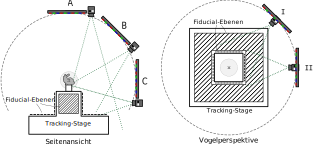
\includegraphics[width=\textwidth]{../graphics/position/stage_views.svg}  

    \caption[Fiducial-Ebenen auf der Tracking-Stage]{Die Fiducial-Ebenen der Tracking-Stage, aus der Seitenansicht (links) und der Vogelperspektive (rechts). 
   Die schraffierten und gestrichelten Flächen sie sind so ausgerichtet, dass sie sich immer im Frustum der Kamera befinden, wenn der Bildschirm auf einer Halbkugel rund um die Szene bewegt wird.
    Abhängig von der vertikalen ($A$, $B$, $C$) und der horizontalen ($I$,$II$) Ausrichtung liegen immer eine, zwei oder drei Ebenen im Frustum der Kamera.
}
    \label{fig:stage_views}
   \end{figure}
 
   Die Marker sind, wie in Abbildung \ref{fig:stage_views}) dargestellt, auf mehreren orthogonalen Flächen (``Fiducial-Ebenen'') angeordnet.
   Die genaue Anzahl und Position der Fiducials ist für die geometrische Betrachtung zunächst unwichtig. 
   In der Seitenansicht ist zu erkennen, dass in jeder der Positionen $A$, $B$ und $C$ mindestens eine der Ebenen im Frustum der Webcam liegt.
   Die Kamera ist dazu wie dargestellt an der Unterseite des Bildschirms angebracht, da sie so am Besten zu den Ebenen ausgerichtet ist. 
   Der Benutzer kann mit dieser Anordnung den Bildschirm um die Szene herum bewegen, und eine halbkugelförmige Lichtfläche erzeugen. 
   Je nach Öffnungswinkel (Field of View) der Kamera können dabei auch niedrigere Beleuchtungswinkel erreicht werden, sodass mehr als die obere Hälfte der eingehenden Beleuchtung erzeugt werden kann.
   
  
      
  \section{Auswahl der Fiducials}
   
   In dieser Arbeit wird ARToolKit zur Positionsberechnung verwendet. Das Programm kann mit beliebig vielen Fiducials gleichzeitig umgehen, die dabei beliebig in der Welt angeordnet sein dürfen.
   Sobald mindestens ein Marker im Kamerabild sichtbar ist, kann auch die Position berechnet werden.
   Damit die Fiducials dabei identifiziert werden können, müssen sich ihre Muster alle unterscheiden.
   
   Da für die Tracking-Stage sehr viele Marker benötigt werden, macht es Sinn sie automatisch zu generieren.
   Dazu wurde die Musterfläche der Fiducials in 4x4 Zellen eingeteilt, wobei jede Zelle entweder schwarz oder weiß sein darf.
   Ein Muster kann so ganz einfach mit einer 16 Bit Ganzahl dargestellt werden. 
   Eine größere Mustermenge lässt sich dann mit einem Pseudo-Zufallsgenerator erzeugen.
   Man muss dabei lediglich darauf achten, dass keine rotationssymmetrischen Muster mit in die Menge aufgenommen werden.
   Da so insgesamt $2^{14}$ unterschiedliche Muster möglich sind, kann man die Menge auch noch weiter eingeschränken:
   Man kann beispielsweise erzwingen, dass sich alle Muster in einer Mindestanzahl an Zellen unterscheidet (hier: 6 Zellen), wodurch sie dann beim Tracking besser auseinandergehalten werden können.
   Abbildung \ref{fig:fiducial_panel} zeigt die ersten 24 Fiducials der so generierten Mustermenge.

  \begin{figure}[H]
   \centering
   
\includegraphics[width=0.6\textwidth]{../graphics/position/fiducial_panel_large.svg}
    \caption[Generierte Fiducials]{Die ersten 24 der algorithmisch generierten Fiducials. Die 16 Zellen werden mit binärzahlen dargestellt, und mit einem Zufallsgenerator erzeugt. } 
   \label{fig:fiducial_panel}
   \end{figure}

% größe vs. anzahl: noise
   Es ist klar dass ein Fiducial, das im Kamerabild eine größerer Fläche aufweist, robuster gegen Sensorrauschen ist ein ein kleineres:
   Je länger die Umrisslinien der Fiducials im Bild sind, desto mehr Pixel sind beim Berechnen der Eckpunkte beteiligt, und desto weniger Einfluss hat das Rauschen einzelner Sensorpixel auf das Ergebnis.
   Sind die Marker kleiner, so lassen sich allerdings auch deutlich mehr davon auf der selben Fläche unterbringen.
   Durch berechnen des Durchschnittwerts beim Auswerten der Position erhöht sich die Genauigkeit wieder.
   Um das Verhalten dieses Tradeoffs zu analysieren wurde eine einfache Testreihe aufgestellt.
   Dabei wurde untersucht, wie sich ARToolKit bei unterschiedlichen Fiducialkonfigurationen verhält.
 
% beschreibung testreihe
\begin{figure}[h]
    \centering

   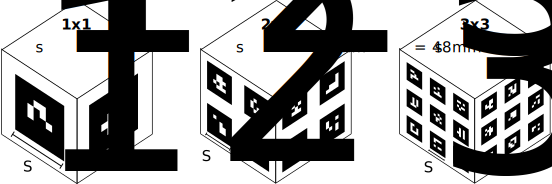
\includegraphics[width=0.65\textwidth]{../graphics/position/testcube_sides.svg}
    \caption[Fiducials der Testreihe]{ Die Fiducial-Testreihe besteht aus drei verschiedenen Konfigurationen, die jeweils aus zwei orthogonalen Ebenen (15x15 cm) bestehen. Darauf befinden sich entweder 1, 4 oder 9 Muster unterschiedlicher Größe.
      Sie wurden so gewählt dass jede Konfigurationen die gleiche Fläche beansprucht, und die Marker dabei noch von einem weißen Rand umgeben sind, sodass sie auch erkannt werden können.
    } 
    \label{fig:testcube_sides}
   \end{figure}

  In der Testreihe werden die drei Musterkonfigurationen 1x1, 2x2 und 3x3 (Abbildung \ref{fig:testcube_sides}) untersucht. 
   Jede Konfiguration besteht aus zwei Panels mit der Größe 15x15 cm, die im rechten Winkel zueinander angeordnet sind.
   Die Fiducials wurden mit einem Laserdrucker ausgedruckt und auf den Seiten eines 15cm Holzwürfels aufgeklebt, wobei sich die zwei Panels einer Konfiguration an einer Kante berühren.
   Der Würfel wurde dann auf eine drehbare Plattform platziert und mit einem Abstand von 50 cm vor der Webcam aufgestellt.
   Es wurde innerhalb von sechs Sekunden von der Frontalansicht des eine Panels, auf die Frontalansicht des anderen rotiert ($0^\circ - 90^\circ$).
   In den Positionen  $0^\circ$,  $45^\circ$ und $90^\circ$ wurde die Bewegung kurz unterbrochen, um die Auswirkungen von Motion-Blur erfassen zu können.
   
   Abbildung \ref{fig:marker_size} zeigt den Abstand zwischen der Kamera und dem Mittelpunkt des Würfels, der von ARToolKit anhand der Marker berechnet wird. 
   Darunter ist jeweils die Anzahl der bei der Berechnung verwendeten Fiducials dargestellt. 
 
 \begin{figure}[h]
    \centering


     \begin{tabular}{cc}% m{0.2\textwidth} m{0.8\textwidth} }
& 
 \begin{tabular}{ccccc}
 \includegraphics[width=0.12\textwidth]{../graphics/position/testcube_1x1_0_cropped.jpg}  & 
  \includegraphics[width=0.08\textwidth]{../graphics/position/testcube_arrow.png} &
\includegraphics[width=0.12\textwidth]{../graphics/position/testcube_1x1_45_cropped_noshift.jpg}  &
  \includegraphics[width=0.08\textwidth]{../graphics/position/testcube_arrow.png} &
\includegraphics[width=0.12\textwidth]{../graphics/position/testcube_1x1_90_cropped.jpg} \\
\end{tabular}
\\
    \includegraphics[width=0.15\textwidth]{../graphics/position/testcube_1x1_45_cropped.jpg} &
    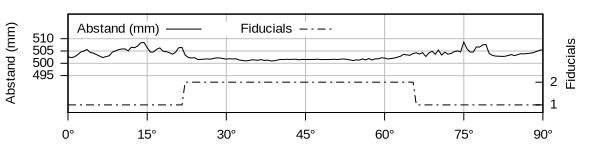
\includegraphics[width=12cm]{../graphics/position/graph_marker_eval_1x1.svg}\\

   \includegraphics[width=0.15\textwidth]{../graphics/position/testcube_2x2_45_cropped.jpg} &
   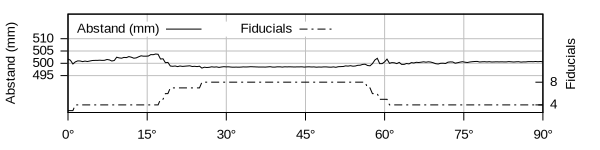
\includegraphics[width=12cm]{../graphics/position/graph_marker_eval_2x2.svg} \\

    \includegraphics[width=0.15\textwidth]{../graphics/position/testcube_3x3_45_cropped.jpg} &
   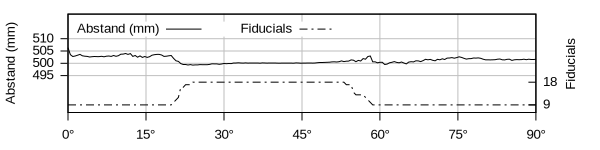
\includegraphics[width=12cm]{../graphics/position/graph_marker_eval_3x3.svg}  

   \end{tabular}

    \caption[Evaluation der Fiducialgröße]{ Drei Musterkonfigurationen auf einem 15 cm großen Würfel werden mit ARToolKit getracked.
  Der Würfel wird dabei langsam um 90 Grad um die senkrechte Achse gedreht. Die Diagramme zeigen den Abstand zum Mittelpunkt des Würfels, sowie die Anzahl der Fiducials die bei der Berechnung verwendet wurden. 
   Bei jeder Konfiguration ist zu sehen, dass der Abstand deutlich genauer berechnet werden kann, sobald Fiducials von beiden orthogonalen Ebenen sichtbar sind. 
    Motion-Blur scheint bei der langsamen Bewegung keinen Einfluss zu haben.
    Man sieht auch, dass es von Vorteil ist, wenn man viele kleine, anstatt wenige große Fiducials verwendet:
     Je mehr Marker im Bild sind, desto geringer sind die Auswirkungen des Sensorrauschens.
    }  

    \label{fig:marker_size}
   \end{figure}

% fazit testreihe

   Mit der Testreihe konnte gezeigt werden, dass viele kleine Marker einen Vorteil gegenüber wenigen, großen Markern besitzen.
   Aus diesem Grund werden auf den Fiducial-Ebenen der Tracking-Stage möglichst viele, kleine Marker aufgebracht. 

  \section{Konstruktion}  
    
    Bei der mechanischen Konstruktion der Fiducials ist es von höchster Bedeutung dass enge Toleranzen eingehalten werden.
    Wenn die tatsächliche Position, Größe oder Orientierung der Fiducials von der Definition abweicht kann ARToolKit die absolute Position nicht korrekt berechnen.
    Insbesondere hängt das Ergebnis auch davon ab, welche Marker konkret bei der Berechung verwendet wurden. 
    Da bei der Tracking-Stage zu jedem Zeitpunkt immer nur ein Teil aller Fiducials sichtbar ist, kommt es bei gleichmäßigen Bewegungen zu starken Sprüngen. 
    Beim Entwurf der Tracking-Stage wurde deshalb darauf geachtet, dass die Fiducials mit Toleranzen im Bereich von $\pm$ 0.5mm im Raum angeordnet werden können.

    Die Basis des Aufbaus besteht aus einer 50x60cm großen, 2mm starken Glasplatte aus einem Bilderrahmen, welche die horizontale Fiducial-Ebene darstellt.
    Die Muster können mit einem gewöhnlichen Laserdrucker auf Papier ausgedruckt werden und ganz einfach auf die Glasplatte geklebt werden.
    Dabei ist es wichtig dass sie flächig aufgeklebt werden, da sich das Papier bei Luftfeuchtigkeitsänderungen  ausdehnen und zusammenziehen kann.
    Die Glasplatte steht auf mehreren identischen Plastikbechern  wird mit zwei LED-Lampen von unten beleuchtet.
    In der Mitte steht eine Holzkiste (15x15x15 cm), deren Boden und Seitenwände ausgesägt wurden..
    Sie ist mit Acrylglasplatten versehen, auf denen die vier vertikalen Fiducial-Ebenen aufgeklebt sind.
    
   \begin{figure}[h]
    \centering
    \includegraphics[width=0.9\textwidth]{../graphics/position/stage_drawing.svg}
    \caption[Aufbau der Tracking-Stage]{Aufbau der Tracking-Stage: Eine Glasplatte, aufgebockt auf Plastikbechern, stellt die Basis dar. Die Fiducials sind auf Papier ausgedruckt und auf die Glasplatte aufgeklebt.
     In der Mitte befindet sich eine Holzkiste mit ausgesägten Seitenwänden, auf der die vertikalen Fiducials mit Acrylglasplatten befestigt sind.
     Mit mehreren Lampen wird der ganze Aufbau von innen beleuchtet, Streulicht wird dabei von blickdichtem Stoff abgefangen.}
    \label{fig:stage_drawing}
   \end{figure}

  \begin{figure}[h]
    \centering
    \includegraphics[width=0.47\textwidth]{../graphics/position/stage_day.jpg}
    \includegraphics[width=0.47\textwidth]{../graphics/position/stage_night.jpg}
    \caption[Fotos der Tracking-Stage]{Die Tracking-Stage, einmal unter einer Bürobeleuchtung und einmal im dunkeln. Die Lampen sind in beiden Bildern auf die gleiche Helligkeit eingestellt.}
    \label{fig:stage_fotos}
   \end{figure}

%inverted
%  \begin{figure}[h]
%   \centering
%   
\includegraphics[width=0.4\textwidth]{../graphics/position/stage_fiducials.svg}
%    \caption[Fiducials der Tracking-Stage]{Die fünf Ebenen der Tracking-Stage: Die Fiducials sind 30x30 mm groß. Die horizontale Ebene (links) besitzt insgesamt 32 Marker und misst 45x45 cm. Die vier vertikalen Ebenen (rechts) sind 15x15 cm groß, und tragen jeweils vier Fiducials. Die Marker sind farblich invertiert.}
%   \label{fig:stage_fiducials}
%   \end{figure}
     Die Fiducials der Tracking-Stage werden vor dem Ausdrucken farblich invertiert, da sie sich so besser zum Durchleuchten eignen.
    ARToolKit kann ein Fiducial nämlich nur dann erkennen, wenn es von einem weißen Rand umgeben ist.
    Invertiert man die Muster und den Webcamstream, so muss der weiße Rand nicht beleuchtet werden. 
    Die zu beleuchtende Fiducial-Fläche ist somit kleiner, wodurch weniger Licht in den Raum abgestrahlt wird.
    Die Fiducial-Ebenen der Tracking-Stage sind in Abbildung \ref{fig:stage_fiducials} im Anhang dargestellt.

  
  \section{Evaluation: Tracking-Stage}
    In diesem Abschnitt wird untersucht, wie gut sich die Tracking-Stage mit ihren beleuchteten Fiducials zur Positionsbestimmung im Dunkeln eignet. 
    Dazu wurde der Laptopbildschirm an drei Positionen bewegt, und so ausgerichtet, wie es bei einer Beleuchtung der Fall ist. 
    Die horizontale und vertikale Ausrichtung des Bildschirms entspricht den Positionen \textbf{BI}, \textbf{CI} und \textbf{CII}  aus Abbildung \ref{fig:stage_views}.
    In jeder Position wurde das Gerät einmal von Hand gehalten, und einmal stationär aufgestellt, wobei versucht wurde einen Abstand von 50 cm einzuhalten.
    Es wurden jeweils eine zwei Sekunden lange Videosequenz aufgezeichnet, und mit ARToolKit die Kameraposition berechnet.
    In den Diagrammen in Abbildung \ref{fig:stage_graphs} ist der so berechnete Abstand zwischen Webcam und dem Weltursprung in Millimeter abgetragen.
    
   \begin{figure}[H]
    \centering
   \begin{tabular}{lr}
    \includegraphics[width=0.24\textwidth]{../graphics/position/trackimg_stationary_B.png} & 
   \includegraphics[width=0.75\textwidth]{../graphics/position/graph_stage_eval_both_B_0_distance.svg} \\
    \includegraphics[width=0.24\textwidth]{../graphics/position/trackimg_stationary_C.png} &
   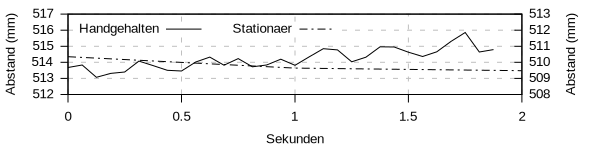
\includegraphics[width=0.75\textwidth]{../graphics/position/graph_stage_eval_both_C_0_distance.svg} \\
    \includegraphics[width=0.24\textwidth]{../graphics/position/trackimg_stationary_C2.png} &
    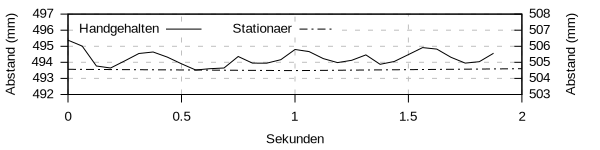
\includegraphics[width=0.75\textwidth]{../graphics/position/graph_stage_eval_both_C2_0_distance.svg} \\
   \end{tabular}
    \caption[Evaluation der Tracking-Stage]{Positionsberechnung im Dunkeln: Die Diagramme zeigen die berechnete Distanz zwischen der Laptopkamera und dem Weltursprung in Millimeter. 
     Es wurden dazu eine Videosequenz aus drei unterschiedlichen Blickwinkeln aufgenommen, wobei der Laptop einmal von Hand gehalten, und einmal stationär betrieben wurde. 
     Die Bilder auf der linken Seite zeigen ein Frame des invertierten Webcamstreams. 
    Es ist gut zu erkennen, dass im handgehaltenen Fall die Position um wenige Millimeter schwankt, was auf ein Verwackeln durch den Benutzers zurückzuführen ist. 
    Im stationären Fall ist sie dagegen sehr stabil, das Sensorrauschen scheint keinen merklichen Einfluss zu haben.
    Man sieht, dass die Positionsberechnung nicht immer exakt möglich ist: Im mittleren Graph driftet die Position im stationären Fall um rund einen Millimeter ab. Die Kamera wurde dabei nicht bewegt, weshalb dieser
    Effekt auf Ungenauigkeiten im Aufbau und Abweichungen in den Kameraparametern zurückzuführen ist.
 
       }  

    \label{fig:stage_graphs}
   \end{figure}

   
    Zusammenfassend lässt sich sagen, dass mit ARToolKit und der Tracking-Stage eine ausreichend genaue Positionsberechnung möglich ist. 
    Im weiteren Verlauf kann davon ausgegangen werden, dass die Position der Webcam bei der Beleuchtung zu jedem Zeitpunkt berechnet werden kann.
 
